\newslide{Schematics -- Identification and Amplifier}{
	\begin{block}{}
	%\centering
		\begin{tikzpicture}
			\node [] (complete) {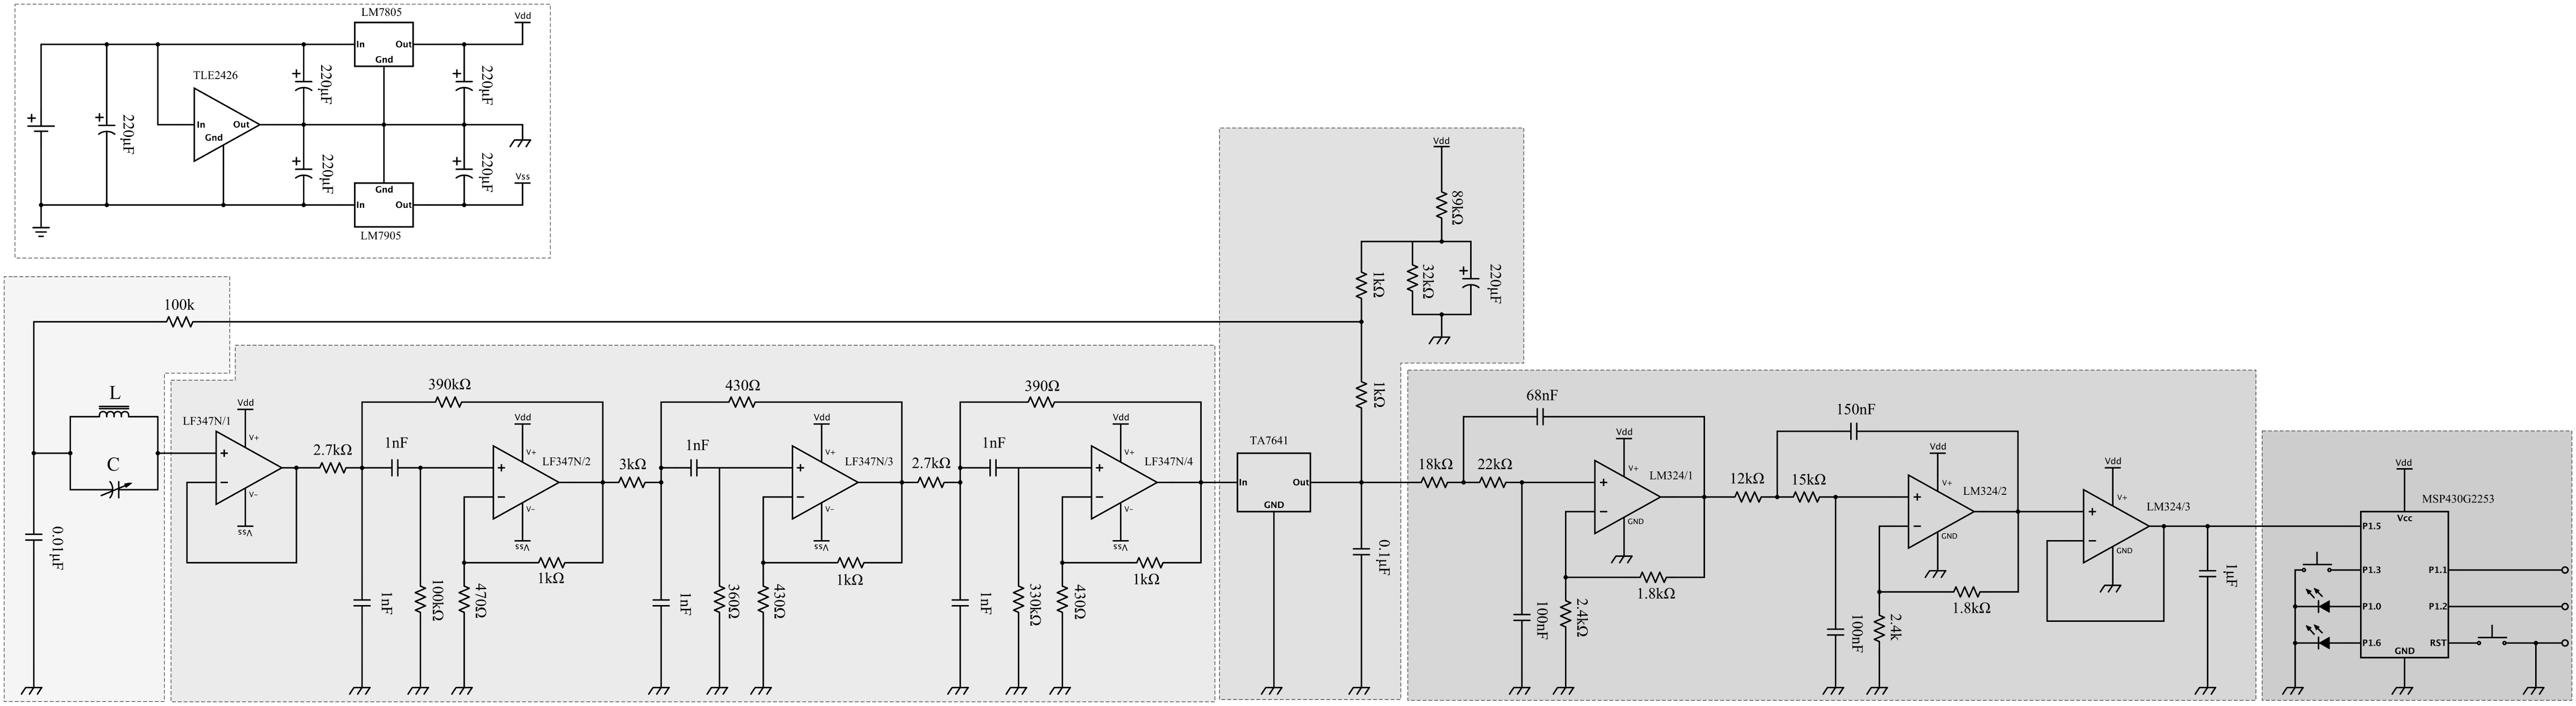
\includegraphics[width=12cm]{img/receiver.png}};
			\node [rectangle,draw, dashed, minimum width=4.85cm, minimum height=2.75cm, xshift=2.1cm, yshift=-0.3cm] (lookat) {};
			\node [rectangle,draw, dashed, at=(complete.south west), anchor=north west, yshift=-1cm] (part2) {
\includegraphics[width=12.5cm]{img/receiver_2.png}};
			\draw [dashed](lookat.south west) -- (part2.north west);
			\draw [dashed](lookat.south east) -- (part2.north east);
			\node [at=(part2.east), anchor=west] (graph) {
			\begin{tikzpicture}

				\begin{semilogxaxis}[xlabel={\scriptsize Frequency (Hz)}, ylabel={\scriptsize Magnitude (dB)},
				                     xmin=10^0, xmax=10^4, ymin=-150, ymax=40, tick label style={font=\scriptsize}, 
				                     height=6cm, width=6cm, grid=both,, grid style={color=gray!50, dotted},
				                     xminorticks=true, scaled ticks=true,log basis x=10,enlargelimits=false,title={Amplifier Characteristic}]
					\addplot[mark=none,line width=1.5] file {../ch2/img/filter2.txt};
				\end{semilogxaxis}
			
			\end{tikzpicture}
			};
		\end{tikzpicture}
	\end{block}
}